\title{Algebra-Based Physics-1: Mechanics (PHYS135A-01): Midterm 1}
\author{Dr. Jordan Hanson - Whittier College Dept. of Physics and Astronomy}
\date{\today}
\documentclass[10pt]{article}
\usepackage[margin=1.5cm]{geometry}
\usepackage{outlines}
\usepackage{graphicx}
\usepackage{amsmath}

\begin{document}
\maketitle

\section{Memory Bank}

\begin{itemize}
\item Unit conversions: 1 km = 1000 m, 1 m = 100 cm, 1 hr = 3600 s, 1 year = $\pi \times 10^7$ s, 1 g/cm$^3$ = 1000 kg/m$^3$.
\item $\vec{x} = a \hat{i} + b\hat{j}$ ... Component form of a two-dimensional vector.
\item $|\vec{x}| = \sqrt{a^2+b^2}$ ... Pythagorean theorem for obtaining vector magnitude.
\item $\theta = \tan^{-1}(b/a)$ ... Obtaining the angle between vector and x-axis.
\item $a = |\vec{x}|\cos(\theta)$ ... Obtaining the x-component with trigonometry.
\item $b = |\vec{x}|\sin(\theta)$ ... Obtaining the y-component with trigonometry.
\item $\Delta x = \vec{x}_f - \vec{x}_i$ ... Definition of displacement.
\item $\vec{v} = \frac{\Delta \vec{x}}{\Delta t} = \frac{\vec{x}_f - \vec{x}_i}{t_f-t_i}$ ... Definition of velocity.
\item $\vec{a} = \frac{\Delta \vec{v}}{\Delta t} = \frac{\vec{v}_f - \vec{v}_i}{t_f-t_i}$ ... Definition of acceleration.
\item $x(t) = x_i + v t$ ... Velocity is the slope of position versus time.
\item $x(t) = \frac{1}{2} a t^2 + v_i t + x_i$ ... With constant acceleration, position is quadratic.  If $a=0$ this becomes the prior function.
\item $v(t) = v_i + a t$ ... With constant acceleration, acceleration is the slope of velocity.
\item $v^2 = v_i^2 + 2 a \Delta x$ ... The kinematic equation without time, assuming constant acceleration.
\item General set of 2D kinematic equations, assuming gravity provides constant vertical negative acceleration.
\begin{align}
\vec{x}(t) &= (x_i + v_{x,i} t) \hat{i} \\
\vec{y}(t) &= (-\frac{1}{2}g t^2 + v_{i,y} t + y_i) \hat{j} \\
\vec{v}_y &= (v_{i,y} - g t) \hat{j} \\
\vec{a} &= -g \hat{j} \\
T_{tof} &= \frac{2 v_0\sin(\theta_0)}{g} \\
R &= \frac{v_0^2\sin(2\theta_0)}{g} \\
v_{x,i} &= v_0 \cos(\theta) \\
v_{y,i} &= v_0 \sin(\theta)
\end{align}
\item Newton's First Law: If $\vec{F}_{\rm net} = 0$, a system will remain at rest or constant velocity.
\item Newton's Second Law: If $\vec{F}_{\rm net} \neq 0$, $\vec{F}_{\rm net} = m\vec{a}$.
\item Newton's Third Law: $\vec{F}_{\rm 12} = - \vec{F}_{\rm 21}$.
\item $\vec{f} = \mu N \hat{i}$ ... The force of friction in the horizontal direction.
\item $\vec{s} = - k \Delta \vec{x}$ ... The spring force.
\end{itemize}

\clearpage

\section{Estimations and Unit Analysis}

\begin{enumerate}
\item Suppose you are standing at the edge of a canyon.  You clap, and here the sound of the echo off of the other side of the canyon wall about 1.5 seconds later.  You estimate the canyon wall to be about 0.25 km away.  1. What is the speed of sound in meters per second?  2. What is it in kilometers per hour?
\begin{itemize}
\item A: 660 m/s, 2400 km/hr
\item B: 330 m/s, 100 km/hr
\item C: 330 m/s, 1200 km/hr
\item D: 660 m/s, 1200 km/hr
\end{itemize}
\item What is 0.25 m$^3$ in cm$^3$?
\begin{itemize}
\item A: 25 cm$^3$, 360 m/s
\item B: 250,000 cm$^3$, 28 m/s
\item C: 2,500 cm$^3$, 28 m/s
\item D: 25,000 cm$^3$, 360 m/s
\end{itemize}
\item What is 100 km/hour in m/s?
\begin{itemize}
\item A: 360 m/s
\item B: 28 m/s
\item C: 10 m/s
\item D: 1200 m/s
\end{itemize}
\item A long tube from a construction site has a volume of 0.001 m$^3$, and a mass of 9 kg.  Convert the numbers to a density and determine the substance.
\begin{itemize}
\item A: 19 g cm$^{-3}$, tungsten
\item B: 9.0 g cm$^{-3}$, copper
\item C: 2.7 g cm$^{-3}$, aluminum
\item D: 7.9 g cm$^{-3}$, iron
\end{itemize}
\end{enumerate}

\section{Vectors}

\begin{enumerate}
\item $\vec{x}_1$ is a vector with a magnitude of 10 meters and that makes an angle of 30 degrees above the x-axis.  What is $\vec{x}_1$ in component form?
\begin{itemize}
\item A: $\vec{x}_1 = 5\sqrt{3}\hat{i} + 5\hat{j}$
\item B: $\vec{x}_1 = \frac{5}{\sqrt{2}}\hat{i} + \frac{5}{\sqrt{2}}\hat{j}$
\item C: $\vec{x}_1 = 5\hat{i} + 5\hat{j}$
\item D: $\vec{x}_1 = 5\sqrt{3}\hat{i} - 5\hat{j}$
\end{itemize}
\item $\vec{x}_2$ is a vector with magnitude 20 meters that makes an angle of 180.0 degrees with respect to the x-axis.  What is $\vec{x}_2$ in component form?
\begin{itemize}
\item A: $\vec{x}_1 = 20\hat{j}$
\item B: $\vec{x}_1 = 20\hat{i}$
\item C: $\vec{x}_1 = 10\hat{i} + 10\hat{j}$
\item D: $\vec{x}_1 = -20\hat{i}$
\end{itemize}
\item A person goes for a walk.  First, they head East for two blocks. Next, they head North for three blocks.  Finally, they head West for six blocks.  If a block is 500 meters, what is their final location?
\begin{itemize}
\item A: $\vec{x} = -4\hat{i}+3\hat{j}$ (km)
\item B: $\vec{x} = 2\hat{i}+2\hat{j}$ (km)
\item C: $\vec{x} = -2\hat{i}+1.5\hat{j}$ (km)
\item D: $\vec{x} = 8\hat{i}+1.5\hat{j}$ (km)
\end{itemize}
\end{enumerate}

\section{Motion Along a Straight Line}

\begin{enumerate}

\item The position of a particle moving along the x-axis is given by $x(t) = 2.0t-1$ (m).  Which of the following is true?
\begin{itemize}
\item A: The particle has a positive acceleration.
\item B: The particle is stationary.
\item C: The particle has a negative acceleration.
\item D: The particle has a positive, constant velocity.
\end{itemize}
\item (Same $x(t)$ as previous question).  What is the velocity, if time is measured in seconds?
\begin{itemize}
\item A: 2 m/s
\item B: 3 m/s
\item C: 4 m/s
\item D: -1 m/s
\end{itemize}
\item A particle moves along the x-axis according to $x(t) = -2t + 7t^2$.  What is the average velocity between $t=0$ and $t=2$ seconds?
\begin{itemize}
\item A: 4 m/s
\item B: 8 m/s
\item C: 12 m/s
\item D: 16 m/s
\end{itemize}
\item (Same $x(t)$ as previous question).  What is the average acceleration of the particle between $t=0$ and $t=2$ seconds?
\begin{itemize}
\item A: 10 m/s
\item B: 14 m/s$^2$
\item C: 12 m/s$^2$
\item D: 7 m/s$^2$
\end{itemize}
\item A sprinter has a constant acceleration of $5.0$ m/s$^2$.  Suppose she starts from rest.  
\begin{enumerate}
\item How long does it take her to reach her top speed of 10.0 m/s?
\begin{itemize}
\item A: 1 second
\item B: 2 seconds
\item C: 3 seconds
\item D: 4 seconds
\end{itemize}
\item What is her displacement at that time?
\begin{itemize}
\item A: 5 meters
\item B: 10 meters
\item C: 15 meters
\item D: 20 meters
\end{itemize}
\item Suppose she is running the 100 meter sprint.  If she continues at 10.0 m/s for the remainder of the race, what will be her total time?
\begin{itemize}
\item A: 9 seconds
\item B: 10 seconds
\item C: 11 seconds
\item D: 12 seconds
\end{itemize}
\end{enumerate}
\end{enumerate}

\section{Motion in Two and Three Dimensions}

\begin{enumerate}
\item The world record highest basketball shot was made from a height of 162.5 meters above the basketball hoop.  The basketball hoop was placed 75 meters horizontally from the shooter.  What is the horizontal velocity required to make the shot?  That is, assume the shooter shoots the ball with no vertical velocity, only horizontal.
\begin{itemize}
\item A: 5 m/s
\item B: 13 m/s
\item C: 18 m/s
\item D: 25 m/s
\end{itemize}
\item A baseball is hit at a 45 degree angle with respect to the horizontal at 40 m/s.  How far away does it land?
\begin{itemize}
\item A: 120 m
\item B: 140 m
\item C: 160 m
\item D: 200 m
\end{itemize}
\item How long is it in the air?
\begin{itemize}
\item A: 3.5 seconds
\item B: 5.5 seconds
\item C: 2.5 seconds
\item D: 10 seconds
\end{itemize}
\end{enumerate}

\section{Forces}
\begin{figure}
\centering
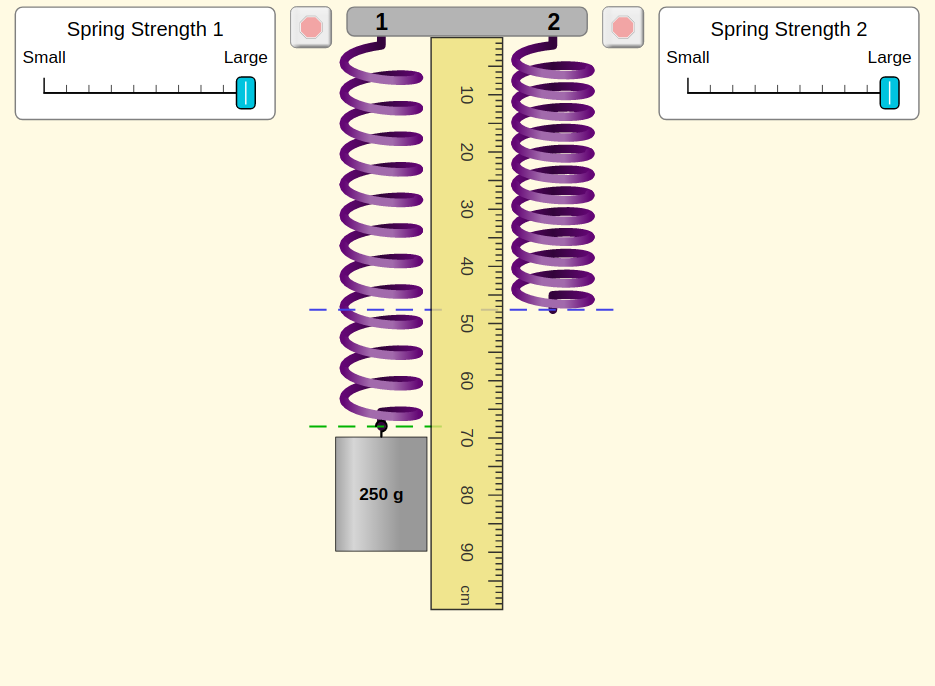
\includegraphics[width=0.4\textwidth,trim=0cm 2cm 0cm 0cm,clip=true]{force_midterm.png}
\caption{\label{fig:force} Two identical springs are shown, each having the same spring constant, $k$.  The left-hand spring has 250 grams hung from it.  The ruler and dashed lines show the stretched and un-stretched lengths.}
\end{figure}
\begin{enumerate}
\item Consider Fig. \ref{fig:force}.  What is the spring constant of these springs?
\begin{itemize}
\item A: 6 N/m
\item B: 8 N/m
\item C: 10 N/m
\item D: 12 N/m
\end{itemize}
\item A man pushes a palette crate across his shop.  He pushes with a force of 75 N.  The mass of the crate is 75 kg.  The coefficient of friction between the crate and the floor is 0.1.  What is the acceleration of the crate?
\begin{itemize}
\item A: 0 m/s$^2$
\item B: 1 m/s$^2$
\item C: 2 m/s$^2$
\item D: 3 m/s$^2$
\end{itemize}
\item \textbf{Bonus} What is an example of a substance that could be added to the floor that would boost the acceleration?
\end{enumerate}

\end{document}